\chapter{Auswertung}
\label{chap7}

Nachdem in den beiden vorangegangenen Kapiteln die Architektur und die Implementierung des entwickelten Kernelmoduls thematisiert wurden, sollen nun die damit
erzielten Ergebnisse diskutiert werden. Dabei wird zunächst in Abschnitt \ref{chap7:synth} ein synthetisches Testszenario betrachtet. Im darauf folgenden
Abschnitt \ref{chap7:boot} wird ein reales Szenario ausgewertet. Abchließend wird in Abschnitt \ref{chap7:mem} sowohl die Rechenlast als auch der
Speicherverbrauch des Moduls untersucht und diskutiert. Für die Tests wurden, sofern nicht anders angegeben, als Festplatte eine Western Digital Raptor
mit 73,4GB Kapazität~\cite{wd:raptor} und als SSD eine Intel X25-E mit 32GB Kapazität~\cite{intel:ssd} genutzt.

\section{Synthetische Leistungsbewertung}
\label{chap7:synth}

Die Leistung des implementierten Kernelmoduls wird in diesem Kapitel anhand eines eigens entworfenen Testszenarios ermittelt. Hierfür wird im ersten
Unterabschnitt zunächst das Testszenario genauer beschrieben. Anschließend werden in Unterabschnitt \ref{chap7:synth:results} die mit Hilfe des Szenarios
gewonnen Testergebnisse vorgestellt und diese abschließend in Unterabschnitt \ref{chap7:synth:discu} diskutiert.

\subsection{Testszenario}
\label{chap7:synth:szenario}

Das synthetische Testszenario, das im Rahmen dieser Arbeit entwickelt wurde, musste zunächst die Hauptanforderung der Vergleichbarkeit der Systemkonfigurationen
erfüllen. Hierfür mussten die Simulationen wiederholbar sein. Neben dieser Hauptanforderung musste es zusätzlich verschiedene Nebenanforderungen erfüllen. Die
Erste besteht darin, die besonderen Eigenschaften eines Caches überhaupt nutzen zu können. Ein gecachtes Medium kann gegenüber einem ungecachten Medium
prinzipbedingt nur einen Geschwindigkeitsvorteil realisieren, wenn auf dieselben Daten mehrfach zugegriffen werden kann. Aus diesem Grund sind die meisten
gebräuchlichen Festplattenbenchmarks bereits ungeeignet. Des Weiteren stellen diese Benchmarks meist ein synthetisches Testszenario dar, welches ebenfalls für
diese Arbeit nicht gewünscht war.

Neben den genannten synthetischen Benchmarks wurde eine andere Möglichkeit in den Arbeiten genutzt, die in Kapitel \ref{chap3} vorgestellt wurde und
vergleichbare Szenarien benötigt. Diese besteht darin, zunächst die Anfragen eines realen Systems an ein Blockgerät aufzuzeichnen. Für den eigentlichen
Benchmark können anschließend die Anfragen an die zu testenden Geräte gestellt und die Verarbeitungszeiten verglichen werden. Dieses Testszenario hat jedoch den
Nachteil, sehr zeitintensiv zu sein, denn zunächst müssen die Daten auf einem Produktivsystem gesammelt werden. Um einen repräsentativen Datensatz zu erhalten
müsste dies über mehrere Tage oder gar Wochen geschehen. Anschließend wären vergleichbare zeitliche Dimensionen nötig, um einen Testlauf durchzuführen. Da im Rahmen
dieser Arbeit mehrere Konfigurationen getestet werden sollten, könnte sich der Zeitbedarf leicht auf Monate summieren. Außerdem würde der Aufbau der nötigen
Infrastruktur zur Aufzeichnung von Datensätzen mit einem nicht vernachlässigbaren Aufwand verbunden sein. Aus diesem Grund konnte dieses Testszenario für diese
Arbeit ebenfalls nicht verwendet werden.

Aus den genannten Gründen ist als Kompromiss ein Zwischenweg aus den beiden genannten Möglichkeiten gewählt worden. Es wurde der synthetische
Benchmark \textit{\mbox{bonnie++}}~\cite{bonnie} hierfür angepasst. \textit{\mbox{Bonnie++}} ist ein synthetischer, auf Dateisystemebene arbeitender, nicht
destruktiver\footnote{Bereits bestehende Daten auf dem Datenträger bleiben erhalten.} Benchmark, welcher Daten auf das zu testende Gerät schreibt und geordnet
und ungeordnet ausliest. Dabei werden die benötigte Zeit und die Prozessorlast gemessen. Da jedoch bei jedem Testlauf die Dateien neu generiert werden mußten,
konnten mit der ursprünglichen Implementierung die Eigenschaften eines Caches nicht genutzt werden. Aus diesem Grund wurde das Programm im Rahmen dieser Arbeit
erweitert, so dass es eine Dateiliste einlesen kann und Lese-/Schreibvorgänge entsprechend dieser Liste durchführt. Dabei besteht die Dateiliste aus mehrere
Zeilen, die wie folgt aufgebaut sind:

\begin{flushleft}
\hspace{0.25cm} \small \texttt{[Dateiname], [Dateigröße], [c|s|d]}
\end{flushleft}

Beim Ausführen von  \textit{\mbox{bonnie++}} wird die Liste eingelesen und je nach dem letzten Parameter die Datei mit der gegebenen Größe erstellt (c), gelesen (s)
oder gelöscht (d). Mit Hilfe dieser Modifikation ließ sich nun ein realitätsnahes Testszenario aufbauen. Um ein reales Desktopsystem zu simulieren, musste
zunächst die Installation und der Bootvorgang simuliert werden. Hierfür wurde als erstes die Datei- und Verzeichnisstruktur eines Ubuntu-Linux-Systems extrahiert
und eine Dateiliste mit dem oben gezeigten Format erstellt, die ihrerseits für das Erstellen von Dateien sorgt. So kann die Installation des Systems simuliert
werden. Die Liste beinhaltet hierbei knapp 121000 Dateien mit einer Gesamtgröße von ca. 3,6GB. Als zweiter Schritt wurde die Menge der gelesen Daten beim Booten
des realen Linux-Systems gemessen. Diese lag bei ca. 150MB. Anschließend wurden aus der Dateiliste des Linux-Systems zufällige Dateien gewählt, die eine
Gesamtgröße von 150MB hatten, und damit eine \textit{\mbox{bonnie++}} Dateiliste erstellt, die das Lesen dieser Dateien durch \textit{\mbox{bonnie++}} veranlasst. Diese
Dateiliste wurde einmalig erstellt und während der Tests nicht verändert. Mit der Liste ließ sich das Booten des Systems und das Starten der Programme annähernd
genau simulieren.

Abschließend musste eine Möglichkeit gefunden werden, das Erstellen, Lesen und Löschen von Nutzerdaten zu simulieren. Hierfür wurden Datenlisten erstellt, die
Angaben zu Dateien mit einer Gesamtgröße von 100MB enthielten. In den Listen überwog dabei die Anzahl von kleinen Dateien stark. Diese Listen wurden
ebenfalls einmalig erzeugt und während der Tests nicht mehr verändert. Bei der Simulation wurden nach jedem simulierten Bootvorgang eine gewisse Anzahl $r$
dieser Sets gelesen, $c\,$ Sets geschrieben und $d$ wieder gelöscht. Dabei wurde die Reihenfolge, welche Sets gelesen, geschrieben oder gelöscht werden,
einmalig festgelegt und ebenfalls während aller Tests nicht verändert. Dieses Vorgehen sollte nun zusammen mit dem Bootvorgang einen Arbeitstag simulieren.

Ausnahmen von dem soeben beschriebenen Vorgehen bildeten die ersten Bootvorgänge einer jeden Simulation. Hierbei wurden jeweils doppelt so viele Sets wie
gewöhnlich geschrieben, bis eine Maximalanzahl $M$ von Sets auf der Festplatte vorhanden waren. Beim Lesen wurden alle Sets berücksichtigt, solange die Anzahl
von Sets auf den Datenträgern den Wert $r$ nicht überstiegen. Des Weiteren wurde beim Erstellen der Erstellungs-, Lese- und Löschreihenfolge der Sets darauf
geachtet, dass immer ein Set existierte, welches an jedem Arbeitstag gelesen wurde. Dieses sollte regelmäßig genutzte Daten simulieren. Die Reihenfolge der
Arbeitstage wurde ebenfalls im Vornherein festgelegt und während der verschiedenen Simulationsläufe nicht verändert. Somit soll an dieser Stelle noch einmal
betont werden, dass alle zufälligen Festlegungen vor dem Beginn der Evaluierung stattfanden.

Bei den konkreten Tests auf einem System galt es jedoch noch eine weitere Funktion des Linux-Systems zu beachten -- nämlich den Datencache im Arbeitsspeicher.
Dieser verzerrte die Messergebnisse des Benchmarkprogramms, da das Betriebssystem den Abschluss von Dateioperationen meldet, obwohl diese noch nicht auf dem
Blockgerät abgeschlossen sind. Weiterhin konnten durch den Arbeitsspeichercache Daten von mehreren Arbeitstagen gehalten werden, so dass z.B. die Daten des Bootens
nicht zwingend vom Blockgerät gelesen wurden sondern aus dem Arbeitsspeichercache. Erste Tests zeigten, dass die Verzerrungen durch diesen Mechanismus enorm
waren und ein Vergleich der verschiedenen zu testenden Konfigurationen nicht möglich war. Zwar war es möglich, die Funktion abzuschalten, was jedoch
zu erheblichen Leistungsverlusten führte, die die Messungen wiederum unrealistisch machten. Das Problem der Übertragung von Daten von einem Bootvorgang zum
Nächsten durch den Arbeitsspeichercache ließ sich durch das Neueinhängen des Blockgerätes in das Dateisystem lösen, da dies das Linux-System dazu veranlasste den
Arbeitsspeichercache zu leeren. Jedoch waren die von \textit{\mbox{bonnie++}} gelieferten Messwerte bezüglich der Leserate ungenau. Um dies Problem zu lösen, wurde als
Maßstab für die Leistung die Zeit zwischen Ein- und Aushängen des Blockgerätes genutzt.

\subsection{Ergebnisse}
\label{chap7:synth:results}

Beim Erstellen einer konkreten Testumgebung sind weitere Dinge zu beachten. Zum einen sollte die gelesene Datenmenge größer sein als der Cache. Ist dies nicht
der Fall, können sämtliche Daten im Cache gehalten werden und es sind keine Rückschlüsse auf die Effizienz des Verdrängungalgorithmuses möglich. Zum anderen ist
die Laufzeit des Tests zu beachten. Wenn von einem momentan üblichen \ac{SSD} und somit auch einer Cachegröße von 32GB ausgegangen wird, würde dies bedeuten,
dass pro simuliertem Arbeitstag mehr als diese 32GB gelesen werden sollten. Das würde zunächst im optimalen Fall bei einer Leserate von 250MB/s und 50
simulierten Arbeitstagen eine Testlaufzeit von ca. zwei Stunden bedeuten. Weiterhin bietet der implementierte Cache sehr viele Freiheitsgrade. Das sind die
Assoziativität, die Cacheblockgröße und die Cacheparameter $m$, $s$ und $i$. Beides in Kombination würde Simulationszeiten von mehreren Monaten bedeuten, sofern
sämtliche Konfigurationskombinationen getestet werden sollten. Dies war im Zeitrahmen dieser Arbeit jedoch nicht möglich. Aus diesem Grund mussten sowohl
Einschränkungen bei der Testumgebung hingenommen werden als auch bei der Anzahl der durchgeführten Simulationen.

Zunächst wurde die Größe des Caches künstlich auf zwei Gigabyte beschränkt. Weiterhin wurde darauf verzichtet, an jedem simulierten Arbeitstag mehr Daten zu
lesen, als der Cache halten kann. Durch eine ausreichend große Anzahl an verschiedenen Datensets auf dem Quellmedium und das Löschen und Schreiben von Sets wurde
jedoch sichergestellt, dass die Datenmenge über mehrere simulierte Tage verteilt größer ist als der Cache. Konkret bedeutet dies Werte von $M=20$, $r=9$, $c=1$
und $d=1$.

Außerdem musste bei den Cacheparametern stark selektiert werden. Dies war notwendig, da die Simulationszeiten starken Schwankungen unterlagen. Beim Erstellen
der Vergleichswerte von der genutzten Festplatte und dem \ac{SSD} kam es zu Abweichungen von bis zu 7,3\% bzw. 9,8\% vom Mittelwert bei Festplatte bzw.
\ac{SSD}. Dies bedeutete, dass jede Konfiguration mehrfach getestet werden musste, um Ausreißer zu vermeiden. Daher wurde zunächst die Blockgröße auf vier
Kilobyte festgelegt. Dies ist die kleinstmögliche sinnvolle Größe, da sie der Blockgröße des verwendeten \ac{ext3} entspricht. Weiterhin wurde der Cacheparameter $m$ auf die Werte $\{4;8;16\}$
beschränkt und die Werte $i$ und $s$ auf $\{1;m\}$. Der Wert von $i=1$ bringt hierbei den Cache näher an einen LFU-Cache und der Wert $i=m$ näher an einen
LRU-Cache. In Abbildung \ref{img:time16} sind die Ergebnisse für $m=16$ dargestellt, wobei für die Assoziativität die Werte
$\{2;4;8;16;32;128;512;2048;8192;32768;131072\}$ genutzt wurden. Für die Werte $m=4$ und $m=8$ konnte die Simulation nur einmal durchgeführt werden, wodurch die
Ergebnisse sehr mit Ausreißern behaftet sind. Aus diesem Grund finden sie sich im Anhang unter \ref{img:time4} und \ref{img:time8}. Wie aus den Diagrammen 
ersichtilich ist, war es lediglich möglich ein spezifisches \ac{SSD} zu nutzen, da sich ansonsten der Testaufwand wiederum verdoppelt hätte.

\begin{figure}[b!]\centering
    \includetikz{figures/chapter7/time16}%
    \caption{Benchmarkergebnisse des Caches für $m=16$}
    \label{img:time16}
\end{figure}

Die Tests konzentrierten sich im weiteren Versuchsaufbau auf die Write-Through-Kon\-fi\-gu\-ra\-tion. Dies liegt zum einen darin begründet, dass die beiden anderen
Konfigurationen nicht im Zeitrahmen dieser Arbeit stabil implementiert werden konnten. So kam es zu sporadischen Synchronisationsproblemen, welche zukünftig noch genauer
analysiert werden müssen. Zum anderen konnten bei stichprobenartigen Tests der Write-Hybrid-Strategie nur unwesentliche Leistungsunterschiede zur
Write-Through-Strategie festgestellt werden. Die Write-Through Strategie lieferte bei der Simulation sehr schlechte Ergebnisse. Die Laufzeit der Simulationen lag
bei allen getesteten Konfigurationen um mehr als das Doppelte über denen der Festplatte. Die genauen Ursachen hierfür werden im Diskussionsteil näher ergründet.

Neben dem Vergleich mit den ungecachten Medien sollte der implementierte Cache zusätzlich mit dem von ZFS verglichen werden. Hierfür wurde die Testumgebung
zunächst für OpenSolaris portiert, da für Linux keine ausgereifte ZFS Implementierung existiert. Anschließend wurden erneut Messwerte für Festplatte und
\ac{SSD} ermittelt, da ein anderes Dateisystem neben der Nutzung eines Caches auch hier eine andere Leistung aufweisen könnte. Wie jedoch in Abbildung \ref{img:time-zfs}
zu sehen ist, war dies nicht der Fall. Anschließend wurde der Test für einen durch das \ac{SSD} gecachten Pool wiederholt. Dieses Ergebnis findet sich ebenfalls
in Abbildung \ref{img:time-zfs} mit dem Messwert für eine Assoziativität von 2048 aus der obigen Messung.

\begin{figure}[b!]\centering
    \includetikz{figures/chapter7/zfs}%
    \caption{Vergleich zwischen dem implementierten Cache und ZFS}
    \label{img:time-zfs}
\end{figure}

Die oben beschriebenen Messungen wurden mit dem sehr performanten Intel-\ac{SSD} durchgeführt. Bei der Simulation mit einem midrange \ac{SSD} (OCZ Vertex Series
32GB~\cite{ocz:ssd}) kam es zu massiven Leistungseinbrüchen. Die Ursache hierfür war in der Größe der Cache\-block\-größe zu finden, welche ungünstig für das
spezifische \ac{SSD} war. Das Diagramm in Abbildung \ref{img:size} zeigt die Leistung des midrange \ac{SSD} in Abhängigkeit von der genutzten Cacheblockgröße.
Die Gründe für die Leistungsunterschiede sollen im nun folgenden Unterabschnitt \ref{chap7:synth:discu} diskutiert werden.

Es konnten im Rahmen dieser Arbeit keine fundierten Messwerte ermittelt werden be\-züg\-lich des Nutzens des \texttt{TRIM}-Kommandos. Dies lag daran, dass lediglich
ein \ac{SSD} zur Verfügung stand, die diese Funktion unterstützt. Bedauerlicherweise konnten mit ihr jedoch keine verwertbaren Messwerte bezüglich der
Cache-Leistung gewonnen werden, so dass auch kein Vergleich zwischen ein- und ausgeschalteter \texttt{TRIM}-Unterstützung ermittelt werden konnte.

\begin{figure}[b!]\centering
    \includetikz{figures/chapter7/size}%
    \caption[Benchmarkergebnisse des Caches für verschiedene Cacheblockgrößen]{Benchmarkergebnisse des Caches für verschiedene Cacheblockgrößen ($m=16$, $s=1$,
    $i=1$)}
    \label{img:size}
\end{figure}

\subsection{Diskussion}
\label{chap7:synth:discu}

Die Ursachen für die Leistungsunterschiede, die im vorangegangenen Abschnitt aufgezeigt wurden, lassen sich über die
verschiedenen internen Blockgrößen und Controller der \acp{SSD} erklären. Abbildung \ref{img:cb} zeigt die Leistung verschiedener \acp{SSD} in Abhängigkeit von
der angeforderten Blockgröße. Es ist klar zu erkennen, dass die Leistung des \ac{SSD}s unter einer individuellen Blockgröße stark sinkt. Dies bedeutet, dass
bei der Wahl der Cacheblockgröße dieser Sachverhalt zu beachten ist. Allerdings kann die Cacheblockgröße nicht ohne weiteres an die native Blockgröße des
jeweiligen \ac{SSD}s angepasst werden. Die Vergrößerung der Cacheblockgröße über das der Dateisystemblockgröße hinaus hat den Nachteil, dass ggf. Daten im Cache
liegen, die nicht benötigt werden. Sollte die Cacheblockgröße z.B. 256kB betragen und eine Datei von vier Kilobyte oft genutzt werden, würde zunächst für diese
Datei ein 256kB Block im Cache eingelagert werden. Im ungünstigsten Fall werden die restlichen 252kB Daten extrem selten bis gar nicht genutzt. Dies könnte z.B.
bei Sicherungskopien der Fall sein. Also würden über 98\% der Daten in diesem Block unnötig vorgehalten werden. Wenn dieses Verhältnis auf den Rest des
Caches übertragen wird, würde im Realfall dieser Wert bei weitem nicht erreicht werden, da es extrem unwahrscheinlich ist, dass die Daten auf dem Quellmedium
entsprechend ungünstig verteilt sind. Es ist jedoch möglich, dass ein nicht unerheblicher Teil des Platzes im Cache blockiert wird, was zu Leistungseinbußen
führt. Dies ist bei der Leistungskurve des zwei Gigabyte Caches zu beobachten. Darum sollte die individuelle Größe der Cacheblockgröße insbesondere bei kleinen
Cachegeräten durch Benchmarks ermittelt werden.

\begin{figure}[b!]\centering
    \includetikz{figures/chapter7/cb}%
    \caption[Datendurchsatz verschiedener SSDs]{Datendurchsatz verschiedener SSDs in Kilobyte pro Sekunde in Abhängigkeit der Blockgröße (Quelle: \textcite{cb} und Eigenmessungen)}
    \label{img:cb}
\end{figure}

Wie in Abbildung \ref{img:time16} zu erkennen ist, hängt die Leistung des Caches bei gleicher Größe in erster Linie von der Assoziativität ab. Es ist mit
Ausnahme der Konfiguration $m=16$, $s=1$, $i=16$ sichtbar, dass die Leistung des Systems mit zunehmender Assoziativität steigt. Dieses Verhalten war zu erwarten,
da bei einer niedrigen Assoziativität die Wahrscheinlichkeit einer Kollision steigt. Bei der Betrachtung des Extremfalls mit einer Assoziativität von eins würden
alle Festplattenblöcke, die voneinander einen Abstand haben, der der Cachegröße entspricht, in den selben Cacheblock fallen. Die Wahrscheinlichkeit, dass dies
passiert, ist sehr hoch und führt zu Leistungseinbußen, da ggf. leere Teile des Caches nicht genutzt werden können. Wenn nun die Assoziativität erhöht wird,
können kollidierende Blöcke eher in einen leeren Bereich des Caches eingelagert werden. Dies ist bei dem anderen Extrem der Fall, bei dem die Assoziativität
genauso groß ist wie der Cache, d.h. der Cache nur aus einem Set besteht. Hierbei kommt es erst zu Verdrängungen, wenn der Cache komplett gefüllt ist. Wie in
Abbildung \ref{img:time16} zu erkennen ist, sinkt die Leistung des Caches ab einem bestimmten Assoziativitätsgrad wieder. Die Ursache hierfür ist die Größe der
Sets. Je größer ein Set ist, umso größer ist der Aufwand, einen Block zu finden, der potentiell in diesem Set liegt. Somit lässt sich ein Tradeoff zwischen
ineffizienter Verdrängung und Rechenleistung feststellten.

Das Abweichen der Konfiguration $s=1$ und $i=16$, lässt sich nicht ohne weiteres erklären, insbesondere da die Simulationen mit $m=4$ und $m=8$ diese Anomalie
bei vergleichbaren Werten für $s$ und $i$ nicht aufweisen. Ganz im Gegenteil, sie zeigen eine ähnliche Anomalie jedoch für andere $s$- und $i$-Werte. Es müsste
zunächst durch längere Simulationen ermittelt werden, ob es sich bei den Messwerten lediglich um statistische Ausreißer handelt oder ob die Ergebnisse
representativ sind. Sollte dies der Fall sein, ist es nötig, dass die genauen Ursachen detailliert untersucht werden. Des Weiteren ist festzustellen, dass
abgesehen von den Anomalien die Manipulation der Werte $s$ und $i$ keine signifikanten Unterschiede liefern. Die Wirkung der Änderung des Wertes $m$ kann nicht
genau bestimmt werden, da die Messwerte bei einer zu hohen Varianz zu dicht beieinander liegen.

Ferner wurde oben festgestellt, dass die Write-Back-Konfiguration eine sehr schlechte Leistung liefert. Die Ursache hierfür ist im Aufbau des Tests zu suchen;
genauer gesagt beim Schreiben neuer Daten. Diese werden sequenziell auf den Datenträger geschrieben, was sowohl bei der Festplatte als auch bei dem \ac{SSD} sehr
schnell vor sich geht. Durch den Write-Back-Cache werden diese sequenziellen Schreibvorgänge jedoch in ungeordnete transformiert. Dies geschieht dadurch, dass
ein Teil des sequenziellen Datenstroms auf das Cachegerät geschrieben wird und der andere Teil direkt auf das Quellgerät. Dies teilt den sequenziellen Datenstrom
zunächst in zwei ungeordnete Datenströme auf, was direkt zu massiven Leistungseinbußen führt, da die Festplatten beim ungeordneten Schreiben signifikant
langsamer werden als beim geordneten. Auch beim \ac{SSD} ist ein ähnliches Verhalten zu beobachten, wenn auch bei weitem nicht im selben Ausmaß. Das Problem wird
jedoch sogar weiter intensiviert, da die Wahrscheinlichkeit groß ist, dass die auf dem Cachegerät eingelagerten Daten zu einem späteren Zeitpunkt wieder auf das
Quellgerät zurückgeschrieben werden müssen. Auch dies geschieht wieder ungeordnet, so dass der ursprünglich gesamte sequenzielle Datenstrom als ungeordneter
Datenstrom auf die Festplatte geschrieben wird.

Abschließend gilt es noch, die Leistung des blockbasierten Caches gegenüber dem Cache des ZFS-Dateisystems zu beurteilen. Es ist in Abbildung \ref{img:time-zfs}
ganz klar und deutlich erkennbar, dass bei guter Wahl der Cacheparameter der blockbasierte Cache dem von ZFS in nichts nachsteht. Ganz im Gegenteil, er kann
sogar einen kleinen Leistungsvorsprung für sich verbuchen. So kann an dieser Stelle festgehalten werden, dass ein blockbasierter Cache gegenüber einem
Dateisystem basierten Cache konkurrenzfähig ist. In Anbetracht dessen, dass der blockbasierte Cache universeller einsetzbar ist, sollte die Nutzung dessen weiter
erforscht werden.

\section{Reale Leistungsbewertung}
\label{chap7:boot}

Nachdem im vorangegangenen Abschnitt die Leistung unter einem synthetischen Test betrachtet wurde, soll in diesem Abschnitt die Leistung unter einem realen Test
bewertet werden. Erneut wird im ersten Unterabschnitt das Testszenario beschrieben, im Zweiten die Ergebnisse dargestellt und im Dritten die Ergebnisse
diskutiert.

\subsection{Testszenario}

Als Testszenario dient der Bootvorgang eines Linux Systems. Dafür wurde die Gentoo-Distribution gewählt, da sich mit ihr der Startvorgang sehr einfach
benutzerspezifisch anpassen lässt. Andere Distributionen, wie z.B. die im vorherigen Kapitel simulierte Ubuntu-Distribution, sind auf Benutzerfreundlichkeit und
einfache Wartung ausgelegt. Hierbei ist eine Anpassung des Bootvorgangs relativ kompliziert, da von den Entwicklern eine weitreichende Nutzeranpassung des
selbigen nicht vorgesehen ist. Bei der Gentoo-Distribution ist dies nicht der Fall, weil sie sich hauptsächlich an Experten wendet und jedes Details des
Bootvorgangs einfach kontrollier- und anpassbar ist.

Für die Leistungsmessung wurde zunächst ein Standardsystem mit Gnome-Desktop installiert. Zur detaillierten Bewertung des Bootvorgangs wurde weiterhin das
Evaluierungsprogramm \textit{Bootchart} \cite{bootchart} installiert. Dieses misst die Zeit zwischen dem Start des \texttt{init}-Programms und des
Login-Bildschirms des Gnome-Desktops. Weiterhin werden Informationen über die Prozessorauslastung, Ein-/Ausgabewartezeiten, Datendurchsatz der Plattengeräte und
deren Auslastung gelogt. Ferner werden die gestarteten Prozesse in Abhängigkeit voneinander dargestellt. Somit ist es möglich den Bootvorgang zu analysieren
und ggf. Leistungsengpässe zu bestimmen.

\subsection{Ergebnisse}

\begin{figure}[b!]
    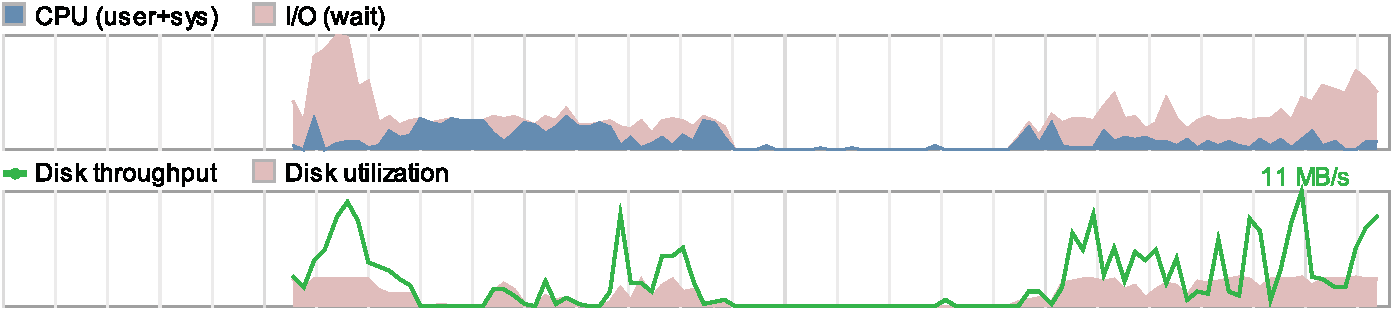
\includegraphics[scale=0.543]{figures/chapter7/boot-hdd}%
    \caption{Leistungsdaten eines HDD-Bootvorgangs}
    \label{img:boot:hdd}
\end{figure}

\begin{figure}[b!]
    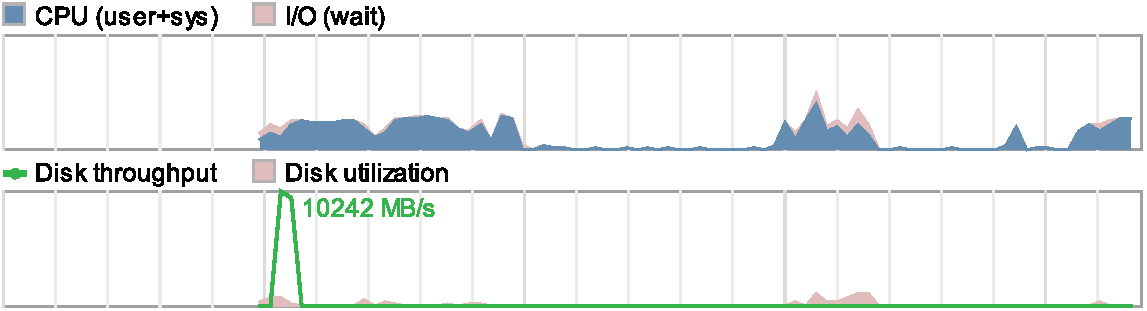
\includegraphics[scale=0.543]{figures/chapter7/boot-ssd}%
    \caption{Leistungsdaten eines SSD-Bootvorgangs}
    \label{img:boot:ssd}
\end{figure}

\begin{figure}[b!]
    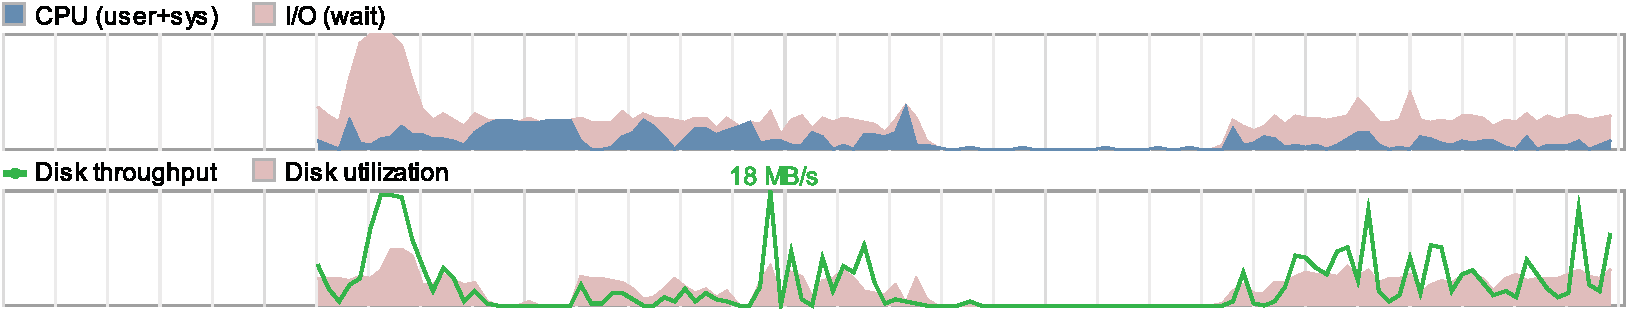
\includegraphics[scale=0.543]{figures/chapter7/boot-cache1}%
    \caption{Leistungsdaten des ersten Cache-Bootvorgangs}
    \label{img:boot:cache1}
\end{figure}

\begin{figure}[b!]
    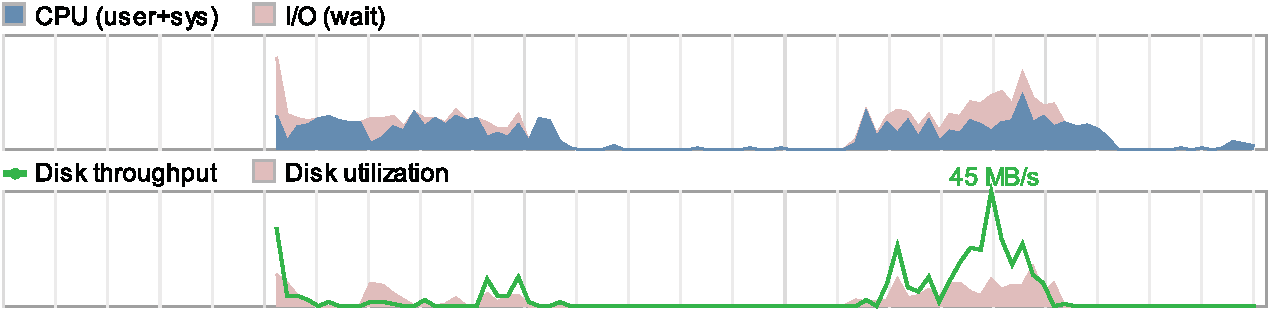
\includegraphics[scale=0.543]{figures/chapter7/boot-cache2}%
    \caption{Leistungsdaten des zweiten Cache-Bootvorgangs}
    \label{img:boot:cache2}
\end{figure}

Die Analyse der Bootvorgänge erfolgte für vier konkrete Szenarien. Es wurde die im letzten Abschnitt erwähnte Western Digital Raptor als Festplatte
und als \acp{SSD} sowohl die OCZ SSD als auch die Intel SSD genutzt. Wobei die Ergebnisse in diesem Unterabschnitt und die Diskussion im nächsten Unterabschnitt
sich auf die Ergebnisse der OCZ \ac{SSD} beziehen. Die Ergebnisse der Intel \ac{SSD} finden sich im Anhang in den Abbildungen \ref{img:bootchart-ssd:intel} bis
\ref{img:bootchart-cache2:intel}.

Es wurden zunächst die Daten für den Bootvorgang eines Systems mit einer herkömmlichen Festplatte ermittelt (Abbildung \ref{img:boot:hdd}). Weiterhin wurden die
Daten für ein identisches System mit einem \ac{SSD} als Bootdatenträger ermittelt (Abbildung \ref{img:boot:ssd}). Abschließend wurden die Werte für das selbe
System mit der Festplatte als Quellmedium und dem \ac{SSD} als Cachemedium aufgezeichnet. Dabei wurden zwei Bootvorgänge betrachtet. Zum einen der Bootvorgang
beim Erstellen des Caches (Abbildung \ref{img:boot:cache1}) und zum anderen der darauf folgende Bootvorgang (Abbildung \ref{img:boot:cache2}). Zur besseren
Übersichtlichkeit sind an dieser Stelle lediglich die Log-Ausschnitte der Prozessorlast und Ein-/Ausgabeaktivität zu sehen, wobei die Breiten der Diagramme
proportional zur Bootzeit sind. Die kompletten Datensätze finden sich im Anhang in den Abbildungen \ref{img:bootchart-hdd} bis \ref{img:bootchart-cache2}.

Des Weiteren wurden die Bootzeiten der verschiedenen Systemkonfigurationen in Abbildung \ref{img:boot:boot} zusammengefasst. Hierbei steht "`Cache 1"' für den
Bootvorgang während des Aufbaus des Caches und "`Cache 2"' für den darauf folgenden.

\begin{figure}[H]\centering
    \includetikz[1.05]{figures/chapter7/boot}%
    \caption{Bootzeiten mit HDD, SSD und Cache als Systemdatenträger}
    \label{img:boot:boot}
\end{figure}

\subsection{Diskussion}

Der Vergleich zwischen den Ein-/Ausgabe-Wartezeiten beim Booten von der Festplatte und dem \ac{SSD} zeigt, dass die Wartezeiten beim Booten von der Festplatte
wesentlich größer sind als die beim \ac{SSD}. Weiterhin ist ein Unterschied beim Datendurchsatz zu erkennen, jedoch muss es sich beim angegebenen
Spitzendurchsatz des \ac{SSD}s von zehn Gigabyte pro Sekunde um einen Auslesefehler handeln. Aus diesem Grund sind diese Werte zwischen Festplatte und \ac{SSD}
nicht vergleichbar. Beim Vergleich dieser Ein-/Ausgabe-Wartezeiten ist zu sehen, dass die Wartezeiten des ersten Cache-Bootvorgangs sich mit denen der
Festplatte ähneln. Sie sind lediglich ein wenig länger, was durch das zusätzliche Schreiben der Bootdaten auf das Cachegerät neben dem Auslesen für den
Bootvorgang erklärt werden kann. Die Wartezeiten des zweiten Bootvorgangs mit Cache ähneln eher denen des \ac{SSD}s, was zu erwarten war, da nach dem ersten
Bootvorgang nahezu alle Anfragen aus dem Cache bedient werden konnten.

In den Abbildungen \ref{img:boot:cache1} und \ref{img:boot:cache2} ist ebenfalls zu erkennen, dass die Prozessorlast nicht wesentlich größer ist als bei den
beiden Bootvorgängen ohne Cache. Dies bestätigt somit die Messungen aus Abschnitt \ref{chap7:synth}.

Bei der Betrachtung der Bootzeiten in Abbildung \ref{img:boot:boot} ist zunächst eine Verlangsamung des Bootvorgangs beim Erstellen des Caches gegebenüber der
Festplatte zu beobachten. Auch dieses Verhalten war zu erwarten, da keine gültigen Daten im Cache vorlagen. Somit konnte der Bootvorgang maximal so schnell
sein, wie derjenige mit der Festplatte. Da jedoch neben dem reinen Auslesen der Bootdaten diese gleichzeitig auf das Quellgerät
geschrieben werden mussten, fiel ein Overhead an, welcher die längere Bootzeit erklärt. Ab dem zweiten Bootvorgang mit Cache konnten die Anfragen jedoch aus
dem Cache bedient werden. Somit verkürzte sich die Bootzeit um 11\% gegenüber der Festplatte und liegt 9\% über der des \ac{SSD}s. Auch in diesem Bereich
spiegeln sich somit die Messergebnisse aus Abschnitt \ref{chap7:synth} wieder.

\section{Ressourcenverbrauch}
\label{chap7:mem}

Da die Nutzung des Caches wenig sinnvoll ist, wenn dieser viele Systemressourcen belegt und somit das System verlangsamt, soll in diesem Abschnitt der
Ressourcenverbrauch näher betrachtet werden. Hierbei wird konkret die Belegung von Rechenkapazität und Speicher genau untersucht.

\subsection{Ergebnisse}

\subsubsection{Prozessorauslastung}

\begin{figure}[b!]\centering
    \includetikz{figures/chapter7/cpu}%
    \caption{Prozessorlast in Abhängigikeit von der Assoziativität}
    \label{img:cpu}
\end{figure}

Ein Maß für die Auslastung wurde ebenfalls mit Hilfe des modifizierten Programmes \textit{\mbox{bonnie++}} ermittelt. Neben dem Datendurchsatz misst
\textit{\mbox{bonnie++}} die Prozessorlast während des Tests. Für die Auswertung der Prozessorlast wurden lediglich die Daten während des simulierten Bootvorgangs
herangezogen, da diese jeweils die stärkste Last aufwiesen. Also sind die Daten der Messung eine Worst-Case-Betrachtung. Die prozentuale Prozessorlast ist im
Diagramm in Abbildung \ref{img:cpu} dargestellt in Abhängigkeit von der Assoziativität. Dabei ist zu beachten, dass eine Last von 100\% die Auslastung einer
CPU bedeutet. Bei einem 4-Kernsystem würde eine Wert von 400\% für eine komplette Auslastung aller Prozessoren stehen. Die Messwerte wurden bei der Simulation mit
den Parametern $m=16$, $s=1$ und $i=1$ ermittelt. Neben der Prozessorlast sind zur besseren Übersicht die Leistungsdaten des Caches aus der Abbildung
\ref{img:time16} mit eingetragen. Diese wurden auf einen Wert von 50 Sekunden normiert.

\subsubsection{Speicher}

Der Speicherverbrauch der ursprünglichen Cacheimplementierung wurde hauptsächlich von den Cacheblock-Metadaten bestimmt. Bei der neuen Implementierung spielen
diese zwar weiterhin eine zentrale Rolle, jedoch wird durch die Iteratorzähler jedes Sets ggf. eine nennenswerte Menge zusätzlichen Speichers belegt je nach
Anzahl der Sets. Dies wird jedoch durch die erhebliche Reduktion des Speicherverbrauchs der Cacheblock-Metadaten überkompensiert. Die Strukturen der beiden
Metadaten sind in den Listings \ref{listing:cache1:block_size} und \ref{listing:cache2:block_size} noch einmal gegenübergestellt, wobei die Kommentare zu jedem
Eintrag durch Größenangaben ersetzt wurden. Es sollte hierbei angemerkt werden, dass die ursprüngliche Implementierung des Caches nicht nur 38 Byte pro
Cacheblock in Anspruch nimmt, sondern 48 Byte. Dies liegt daran, dass auf einem 64-Bit System jedes Element einer Datenstruktur vom GCC-Compiler an eine Adresse,
die ein Vielfaches von acht ist, gelegt wird. Dies Problem hätte jedoch durch eine einfache Compileranweisung behoben werden können, weshalb im Weiteren von
einer Größe von 38 Byte ausgegangen wird.

\lstset{language=C,
		basicstyle=\ttfamily\scriptsize,
		backgroundcolor=\color{lightgray},
		captionpos=b, 
		tabsize=4,
		showstringspaces=false,
		keepspaces=true,
		linewidth=\textwidth,
		xleftmargin=0mm,		
		commentstyle=\color{comment},
		keywordstyle=\bfseries\color{keyword},
		stringstyle=\color{string},
		morecomment=[s][\color{javadoc}]{/**}{*/}}

\hfill
\begin{minipage}{.45\textwidth}
\lstinputlisting[frame=trbl,caption=Gesamtgröße 38 Byte, label=listing:cache1:block_size]{listings/struct_cacheblock1_size.source}
\end{minipage}
\hfill
\begin{minipage}{.45\textwidth}
\lstinputlisting[frame=trbl,caption=Gesamtgröße 8 Byte, label=listing:cache2:block_size]{listings/struct_cacheblock2_size.source}
\end{minipage}\hfill

Der exakte Speicherbedarf lässt sich in Abhängigkeit von Cachegröße, Blockgröße und Assoziativität berechnen. Mit der Formel \ref{eqn:blocks} lässt sich
in einem ersten Schritt die Blockanzahl des Caches berechnen:

\begin{equation}\label{eqn:blocks}
\text{Blockanzahl} \cdot 2^{20} = \frac{\displaystyle \text{Cachegröße [MB]}}{\displaystyle 512\text{B} \cdot \text{Cacheblockgröße}}
\end{equation}

Im Weiteren lässt sich mit der Formel \ref{eqn:size1} der Speicherverbrauch für die Cacheblock-Metadaten der ursprünglichen Implementierung berechnen:

\begin{equation}\label{eqn:size1}
\text{Speicherverbrauch [MB]} = \text{Blockanzahl} \cdot 2^{20} \cdot 38 \text{B}
\end{equation}

\clearpage

Für den Speicherverbrauch der neuen Implementierung müssen zusätzlich die Iterationszähler berücksichtigt werden. Aus diesem Grund erweitert sich die Formel wie
in der Gleichung \ref{eqn:size2} zu sehen ist:

\begin{equation}\label{eqn:size2}
\text{Speicherverbrauch [MB]} = \underbrace{\text{Blockanzahl} \cdot 2^{20} \cdot 8 \text{B}}_{\text{Cacheblock-Metadaten}} + \underbrace{\frac{\displaystyle \text{Blockanzahl} \cdot 2^{20}}{\displaystyle \text{Assoziativität}} \cdot 4 \text{B}}_{\text{Iterationszähler}}
\end{equation}

Zur besseren Veranschaulichung ist in Abbildung \ref{img:memory} der Speicherverbrauch der Cache\-block-Metadaten in Abhängigkeit von der Cachegröße dargestellt.
Für die optimierte Implementierung wurde eine Assoziativität von 2048 angenommen, da sich diese, wie oben diskutiert, als effizient herausgestellt hat. Das Diagramm
stellt dabei den Bedarf für die beiden Cachblockgrößen von 4kB und 128kB dar.

\begin{figure}[t!]\centering
  \includetikz{figures/chapter7/mem}%
  \caption[Speicherverbrauch der Cacheblock-Metadaten]{Speicherverbrauch der Cacheblock-Metadaten in Abhängigkeit von der Cachegröße}
  \label{img:memory}
\end{figure}

\subsection{Diskussion}

Das Diagramm der Prozessorlast in Abbildung \ref{img:cpu} verdeutlicht das in Abschnitt \ref{chap7:synth} bereits angesprochene Problem der steigenden
Prozessorlast bei größer werdender Assoziativität. Demzufolge kann festgestellt werden, dass es sinnvoll ist für jedes System das optimale Assoziativitätsmaß zu
finden. Weiterhin ist ersichtlich, dass sich die Prozessorlast bezogen auf einen Kern bei optimaler Assoziativität  zwischen 10\% und 20\% bewegt, bei nahezu
vollständiger Auslastung des Cachegeräts. Dieser Wert ist gut akzeptierbar, insbesondere da dies bei einem modernen 4-Kern System eine Gesamtsystemlast
von weniger als 5\% bedeutet. Folglich steht der Nutzung des Caches aus Sicht der Prozessorauslastung nichts im Wege.

Weiterhin gilt es den Speicherverbrauch des Caches zu beurteilen. Hierbei kann zunächst festgestellt werden, dass durch die Optimierungen, die an der
\textit{dm-cache} Implementierung im Rahmen dieser Arbeit durchgeführt wurden, selbst im ungünstigsten Szenario einer Assoziativität von lediglich eins, der
Speicherverbrauch um knapp 70\% gesenkt wurde. Dies zeigt die folgende Rechnung:

\[
\begin{split}
\text{Blockanzahl} \cdot 2^{20} \cdot 38 \text{B} & \stackrel{?}{>} \text{Blockanzahl} \cdot 2^{20} \cdot 8 \text{B} + \max_\text{Assoziativität} \left\{
\frac{\displaystyle \text{Blockanzahl} \cdot 2^{20}}{\displaystyle \text{Assoziativität}} \cdot 4 \text{B} \right\} \\
\text{Blockanzahl} \cdot 2^{20} \cdot 38 \text{B} & \stackrel{?}{>} \text{Blockanzahl} \cdot 2^{20} \cdot 8 \text{B} + \frac{\displaystyle \text{Blockanzahl} \cdot 2^{20}}{\displaystyle 1} \cdot 4 \text{B}\\
38 \text{B} & > 12 \text{B}\\
\end{split}
\]

Wie Abbildung \ref{img:memory} zu entnehmen ist, ist der Speicherverbrauch des Caches bei einem ein Terabyte großen Cache mit einer Blockgröße von vier Kilobyte
ca. zwei Gigabyte groß. Zunächst ist anzumerken, dass es momentan nicht sinnvoll ist, Caches mit mehr als einem Terabyte zu betrachten, da in nächster Zeit
kein solches \acp{SSD} auf dem Consumer-Markt verfügbar sein wird. Der Speicherverbrauch von zwei Gigabyte ist sehr kritisch zu sehen, da dies einen Großteil
des bei aktuellen Systemen verfügbaren Speichers in Anspruch nehmen würde. Jedoch verdeutlichen Abbildungen \ref{img:size} und \ref{img:cb}, dass eine
Blockgröße im Bereich von 128kb-256kB besser geeignet ist, als eine von vier Kilobyte . Hierbei sinkt der Speicherverbrauch auf ca. 128MB bzw. 64MB. Dies
sollte für aktuelle Systeme kein Problem darstellen. Daher kann auch in Bezug auf den Speicherverbrauch festgestellt werden, dass ein blockbasierter Cache
vorteilhaft ist.
